\documentclass[11pt,a4paper]{article}

% English comments only.
\usepackage[a4paper,margin=1in]{geometry}
\usepackage{fontspec}
\usepackage{graphicx}
\usepackage{booktabs}
\usepackage{tabularx}
\usepackage{longtable}
\usepackage{array}
\usepackage{enumitem}
\usepackage{hyperref}
\usepackage{xurl}
\usepackage{fancyhdr}
\usepackage{titlesec}
\usepackage{setspace}
\usepackage{caption}
\usepackage{float}
\usepackage{xcolor}
\usepackage{lastpage}

\setmainfont{Times New Roman}
\setsansfont{Arial Unicode MS}
\setmonofont{Menlo}
\linespread{1.12}
\setlength{\parskip}{0.5em}
\setlength{\parindent}{1.5em}
\setlength{\headheight}{14pt}
\setlength{\emergencystretch}{1.5em}
\setlength{\headheight}{14pt}
\setlength{\emergencystretch}{1.5em}
\hypersetup{
  colorlinks=true,
  linkcolor=black,
  urlcolor=blue!50!black,
  citecolor=black,
  pdftitle={A-CSM: AI Contextual Signal Matrix},
  pdfauthor={ZON RZVN}
}

\pagestyle{fancy}
\fancyhf{}
\fancyhead[L]{A-CSM: AI Contextual Signal Matrix}
\fancyhead[R]{Technical Report v1.0}
\fancyfoot[C]{\thepage}
\renewcommand{\headrulewidth}{0.4pt}
\renewcommand{\footrulewidth}{0pt}

\titleformat{\section}{\large\bfseries}{\thesection.}{0.6em}{}
\titleformat{\subsection}{\normalsize\bfseries}{\thesubsection}{0.6em}{}

\begin{document}

\begin{titlepage}
\centering
{\Large \textbf{A-CSM: AI Contextual Signal Matrix}\par}
\vspace{0.8em}
{\large Technical Report for the Public-Safe Core v0.1.0\par}
\vspace{0.5em}
{\normalsize Conversational Contextual Risk Review After Interaction Artifacts Are Available\par}
\vspace{2em}

\begin{tabular}{rl}
Author: & ZON RZVN \\
Role: & Independent Researcher, Taiwan \\
Version: & Technical Report v1.0 \\
Document date: & 2026-03-18 \\
Project page: & \url{https://rzvn.io/a-csm} \\
Repository: & \url{https://github.com/kyozong77/A-CSM} \\
Reserved DOI: & \texttt{10.5281/zenodo.19097267} \\
Report license: & CC BY-NC-ND 4.0 \\
Repository scope: & Public-safe GitHub core release candidate v0.1.0 \\
\end{tabular}

\vfill

\begin{minipage}{0.9\linewidth}
\small
\textbf{Scope statement.} This report covers only the released public-core implementation in the GitHub upload package for \texttt{v0.1.0}. It describes the executable system that detects conversational contextual risk after interaction artifacts are available. Unreleased or restricted components are outside the scope of this report.
\end{minipage}

\vfill
\end{titlepage}

\begin{abstract}
A-CSM, short for \textit{AI Contextual Signal Matrix}, is the formal title of the released public core. The released core is a deterministic Node.js pipeline for reviewing conversational contextual risk after a dialogue artifact already exists. Its function is narrower than runtime moderation. It serves reproducible baseline validation, release review, red-teaming support, and post-session technical inspection.

This report documents only the public-safe core version, \texttt{v0.1.0}. The scope is restricted to what is present in the GitHub upload folder: input formats, pipeline stages, released configuration surface, output contract, verification path, and current release boundary. Unreleased or restricted components are not discussed.

The current public core accepts structured \texttt{turns} input, top-level \texttt{text} shortcut input, and Markdown transcript input. It runs through a released eight-stage orchestration pipeline that covers de-identification, event detection, VCD inference, repeat-aware ledgering, TAG escalation, \texttt{PS/SUB/F/E} derivation, schema validation, and release-gate evaluation. On the verified publication package dated 2026-03-18, the local test suite passed \texttt{921} tests with \texttt{0} failures, and the published baseline run recorded \texttt{accuracy = 1.0}, \texttt{false\_positive\_rate = 0}, and \texttt{false\_negative\_rate = 0} for the released risk-status baseline slice.

The report has four purposes. First, it states the formal title, scope, and release boundary of A-CSM. Second, it specifies how the released core works and how it should be run. Third, it records what the current verification state does and does not prove. Fourth, it places the released system in relation to CXC-7, CXOD-7, USCH, and the empirical evidence reported by Moore et al. without extending beyond the released package.
\end{abstract}

\noindent\textbf{Keywords:} conversational contextual risk, public-safe release, deterministic pipeline, transcript review, post-session assessment, A-CSM

\tableofcontents
\newpage

\section{Introduction}

Conversational AI safety is often discussed at the level of single outputs. That perspective is useful for refusal behavior, harmful-content filtering, and policy compliance, but it does not fully capture risks that accumulate across interaction history. In multi-turn settings, a conversation may remain superficially coherent while still drifting in ways that matter for user-side safety, context alignment, and system accountability.

The public A-CSM release addresses that narrower but technically important problem. It does not intervene during generation. It operates after interaction artifacts are available. The project page uses the same formal title and presents A-CSM as a risk-focused public release for this line of work.\footnote{\url{https://rzvn.io/a-csm}} The released \texttt{v0.1.0} package is therefore presented here as a review-oriented implementation artifact.

This report limits itself to the GitHub upload folder for the public core release. All claims in the following sections are anchored to the contents of the released repository, the project page, and the specific set of prior papers and standards that the current release already references. It does not extend to future or non-public components.

\section{Public Positioning and Release Boundary}

\subsection{Official Name and Release Identity}

The released system is formally titled \textbf{A-CSM: AI Contextual Signal Matrix}. The repository README describes it as a deterministic Node.js pipeline for assessing conversational AI risk across factual reliability, context alignment, user-side safety, and system accountability dimensions. The same README also states that the repository is a public-safe release candidate intended for external sharing and reproducible baseline validation.

That public identity constrains what the report can claim. The technical report therefore treats \texttt{v0.1.0} as a released system with a clearly delimited function: post-session conversational contextual risk review for the public core package.

\subsection{What the Public Core Includes}

The GitHub upload folder currently includes:

\begin{itemize}[leftmargin=1.8em]
\item a Node.js ES module runtime centered on \texttt{scripts/acsm-orchestrator.mjs},
\item released configuration files and sample inputs,
\item deterministic transcript processing and report generation,
\item validation, regression, and release-gate scripts,
\item documentation for the orchestrator, validation framework, annotation workflow, limitations, and public-claims boundaries,
\item a public baseline package that can be rerun locally.
\end{itemize}

\subsection{What the Public Core Does Not Include}

The same release boundary also excludes several categories of material:

\begin{itemize}[leftmargin=1.8em]
\item private taxonomy,
\item proprietary scoring logic,
\item private evaluation assets,
\item confidential evaluation layers,
\item runtime intervention systems,
\item clinical or legal decision functions.
\end{itemize}

\begin{figure}[H]
\centering
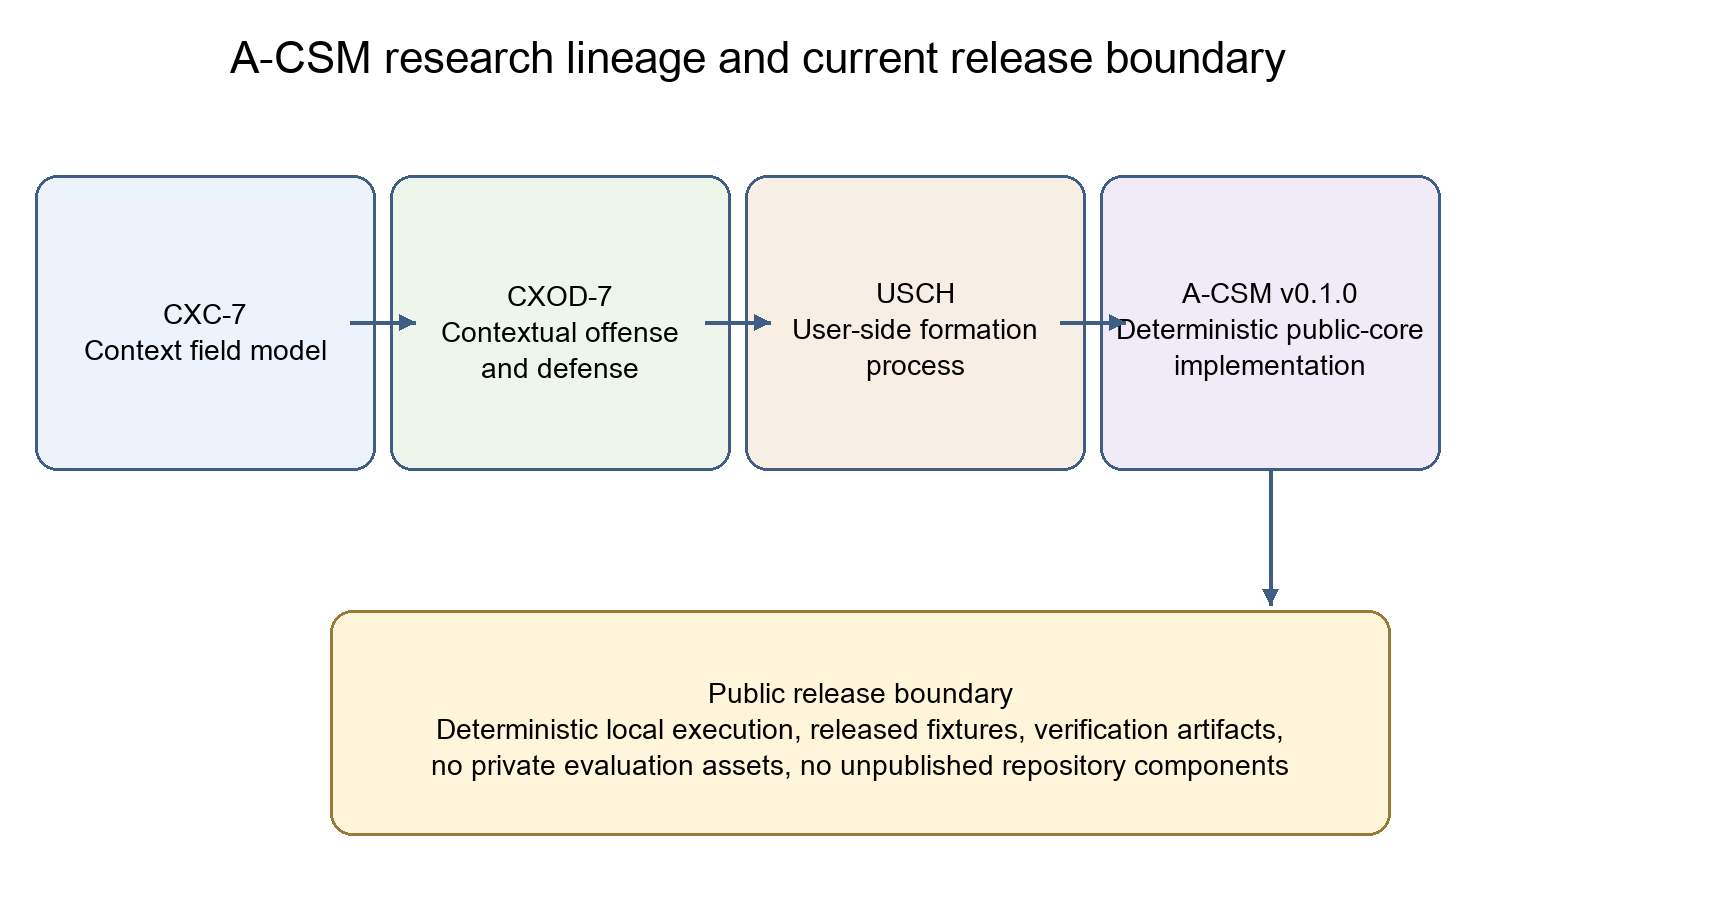
\includegraphics[width=0.9\linewidth]{assets/figure_1_lineage.png}
\caption{Research lineage and public release boundary for the GitHub upload package.}
\end{figure}

\section{System Scope and Core Claims}

\subsection{Problem Definition}

Within the public branch, A-CSM is a post-session system. It accepts a completed interaction artifact and produces a structured review output. The release is concerned with conversational contextual risk rather than isolated text toxicity or benchmark-only performance. The system evaluates risk after a transcript is available, which is why its inputs, traces, and outputs are all organized around the dialogue artifact as a whole.

\subsection{Released Design Principles}

Five design principles are visible in the public branch.

\begin{enumerate}[leftmargin=1.8em]
\item \textbf{Determinism.} The same input and configuration should produce the same result.
\item \textbf{Local execution.} The released scoring path runs without external runtime services.
\item \textbf{Auditability.} Outputs preserve evidence traces and stage-level artifacts.
\item \textbf{Conservative release discipline.} Public claims are limited to what the public branch can demonstrate.
\item \textbf{Human review.} The system supports review and escalation; it does not replace expert judgment.
\end{enumerate}

\subsection{Scope of the Present Report}

The present report is limited to the released GitHub upload package dated 2026-03-18. It does not extrapolate to future releases or to components that are not part of the released repository. The intent is to provide an accurate technical report for the current public-safe core version only.

\section{Architecture and Execution Path}

\subsection{Input Surface}

The public orchestrator supports three input forms:

\begin{itemize}[leftmargin=1.8em]
\item \textbf{\texttt{turns} mode}, where structured JSON turns are provided directly;
\item \textbf{\texttt{text} shortcut mode}, where a top-level text field is normalized into a single-turn conversation;
\item \textbf{Markdown transcript mode}, where \texttt{input-contract} converts \texttt{.md} or \texttt{.markdown} files into stable turns before scoring.
\end{itemize}

This distinction is important because \texttt{input-contract} is a preprocessing boundary for Markdown inputs. It is not itself one of the eight released orchestration stages.

\subsection{Eight Released Stages}

The released orchestrator documentation defines the following eight-stage pipeline:

\begin{enumerate}[leftmargin=1.8em]
\item De-identify transcript content (\texttt{deid-pipeline})
\item Detect four-axis risk events (\texttt{event-engine-v1})
\item Infer VCD defense posture (\texttt{vcd-inference})
\item Build repeat-aware ledgers (\texttt{ledger-repeat-engine})
\item Compute TAG escalation level (\texttt{tag-escalation})
\item Derive \texttt{PS/SUB/F/E} (\texttt{ps-sub-fe-core})
\item Validate USCI schema and invariants (\texttt{schema-invariant-service})
\item Evaluate release gate readiness (\texttt{release-gate})
\end{enumerate}

The public engine inventory currently contains \texttt{43} event-engine rules and a \texttt{20}-rule VCD matrix. The configuration surface controls how those released engines are applied through mappings, thresholds, and rule toggles.

\begin{figure}[H]
\centering
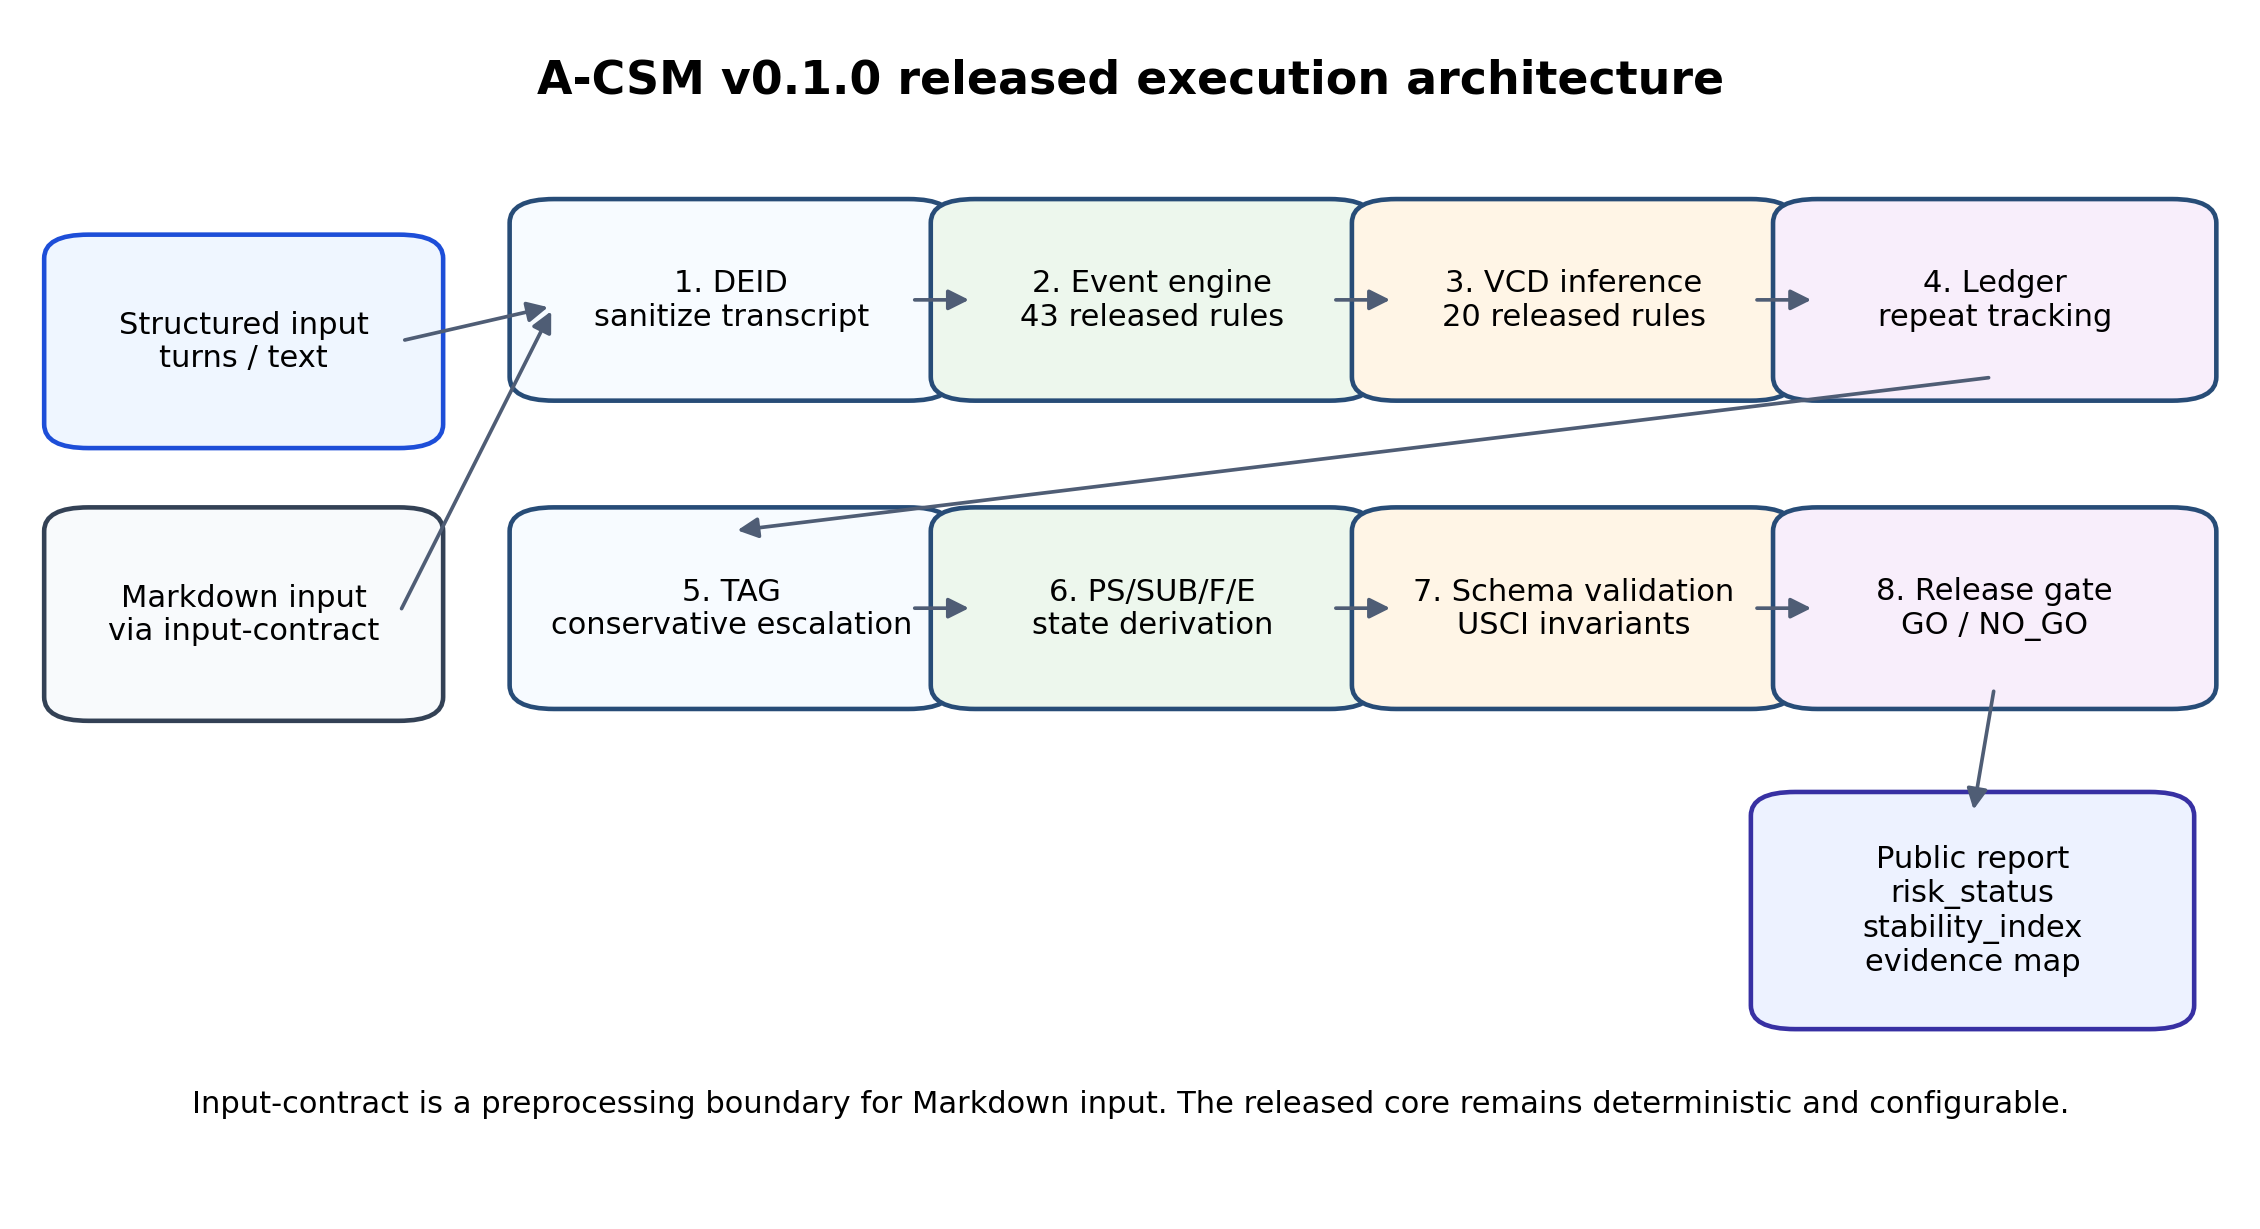
\includegraphics[width=0.95\linewidth]{assets/figure_2_architecture.png}
\caption{Released architecture of the public-safe core \texttt{v0.1.0}.}
\end{figure}

\subsection{Output Contract}

The released report block exposes ten required fields:

\begin{small}
\small
\begin{longtable}{>{\raggedright\arraybackslash}p{0.34\linewidth} >{\raggedright\arraybackslash}p{0.56\linewidth}}
\toprule
\textbf{Field} & \textbf{Released purpose} \\
\midrule
\endhead
\texttt{risk\_status} & Final operational state for the run \\
\texttt{peak\_status} & Highest reached severity during the run \\
\texttt{stability\_index} & Normalized stability score on a 0--100 scale \\
\texttt{evidence\_list} & Ordered evidence items from unified events \\
\texttt{false\_positive\_warnings} & Non-blocking warnings collected across stages \\
\texttt{human\_review\_note} & Mandatory reminder that the output requires human review \\
\texttt{event\_evidence\_map} & Event-to-evidence traceability structure \\
\texttt{confidence\_interval} & Bounded interval on the 0--4 risk scale \\
\texttt{digital\_fingerprint} & SHA-256 fingerprint of sanitized content and derived report \\
\texttt{rule\_version} & Schema and rule-set metadata used during evaluation \\
\bottomrule
\end{longtable}
\normalsize
\end{small}

In addition to the report block, the orchestrator preserves \texttt{summary}, \texttt{steps}, and \texttt{derived} structures. These are part of the technical trace rather than the public-facing summary.

\section{Operational Procedure}

\subsection{Environment and Runtime Requirements}

The public package requires \texttt{Node >= 20}. The released scoring path is local-first and does not depend on external runtime services. Optional Python utilities are included in the repository, but they are auxiliary research helpers and are not required to execute the core orchestrator.

\subsection{Verification Workflow}

The repository README and verification memorandum establish a compact verification path for the released package:

\begin{verbatim}
npm run lint:syntax
npm test
npm run test:coverage
npm run performance:baseline
npm run security:scan
npm run audit:workspace
\end{verbatim}

These commands validate syntax, the Node.js test suite, coverage execution, the published performance baseline, secret scanning, and workspace readiness.

For transcript normalization alone, the repository also provides an explicit input-contract entry point:

\begin{verbatim}
npm run input:check -- \
  --input config/input-contract-input.sample.md \
  --config config/input-contract-config.sample.yaml \
  --output logs/input-contract-result.json \
  --format both
\end{verbatim}

\subsection{End-to-End Execution}

For the JSON sample path, the orchestrator can be run as follows:

\begin{verbatim}
npm run acsm:run -- \
  --input config/acsm-orchestrator-input.sample.json \
  --config config/acsm-orchestrator.json \
  --validation config/validation-runner-result.sample.json \
  --output logs/acsm-orchestrator-result.json \
  --format both
\end{verbatim}

For the Markdown transcript path, the README specifies:

\begin{verbatim}
npm run acsm:run -- \
  --input config/input-contract-input.sample.md \
  --config config/acsm-orchestrator.json \
  --output logs/acsm-orchestrator-from-md.json \
  --format both
\end{verbatim}

The release also includes batch and regression commands:

\begin{verbatim}
npm run acsm:run:200
npm run regression:check
\end{verbatim}

\subsection{Reviewer Checks}

For the public branch, a reviewer should confirm four things:

\begin{itemize}[leftmargin=1.8em]
\item the run completes without runtime or schema failure,
\item the summary exposes release-gate and validation signals,
\item the report block contains the released fields,
\item the stage traces remain available for rerun inspection.
\end{itemize}

\begin{figure}[H]
\centering
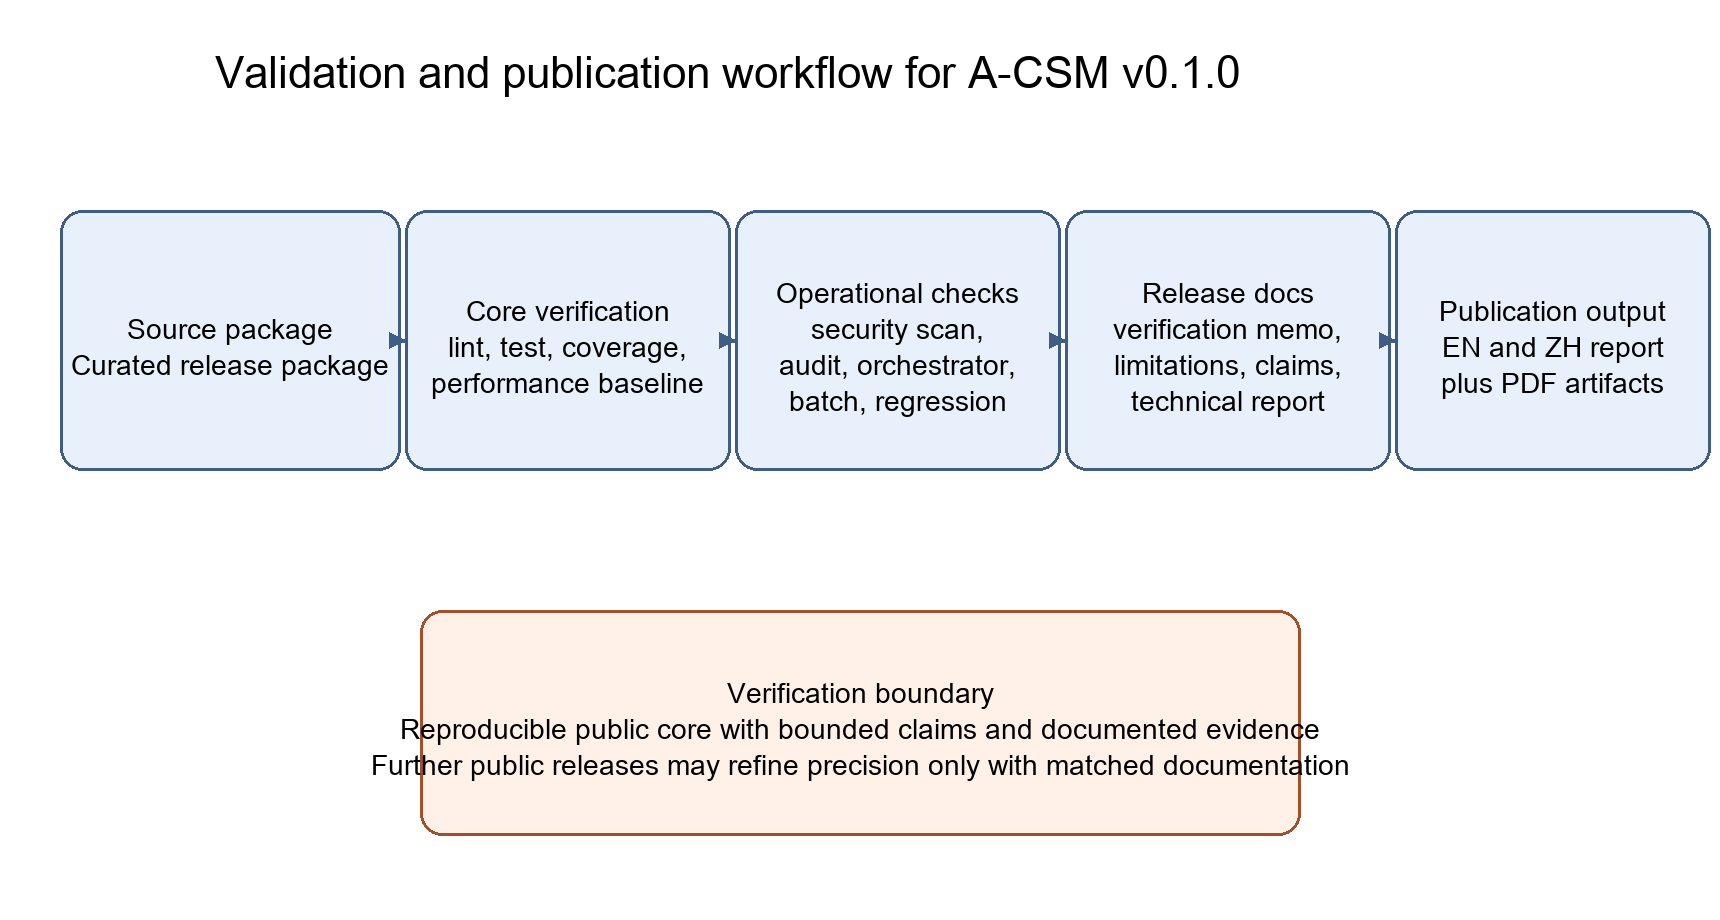
\includegraphics[width=0.92\linewidth]{assets/figure_4_validation_workflow.png}
\caption{Verification and publication workflow for the public-safe core.}
\end{figure}

\section{Current Verification Status of \texttt{v0.1.0}}

\subsection{Repository-Level Results}

The verification memorandum dated 2026-03-18 reports the following local results for the publication package:

\begin{table}[H]
\centering
\caption{Current repository-level verification results}
\begin{tabularx}{\linewidth}{>{\raggedright\arraybackslash}p{0.55\linewidth} >{\raggedright\arraybackslash}X}
\toprule
\textbf{Check} & \textbf{Recorded result} \\
\midrule
\texttt{npm test} & \texttt{921 pass / 0 fail} across \texttt{41} suites \\
\texttt{npm run test:coverage} & Pass \\
\texttt{npm run performance:baseline} & Pass, readiness ready \\
\texttt{npm run security:scan} & No secret findings \\
\texttt{npm run audit:workspace} & READY \\
\texttt{npm run acsm:run} & Pass \\
\texttt{npm run acsm:run:200} & Pass \\
\texttt{npm run regression:check} & Pass \\
\bottomrule
\end{tabularx}
\end{table}

The published performance baseline file records:

\begin{itemize}[leftmargin=1.8em]
\item \texttt{total\_cases = 100}
\item \texttt{exact\_matches = 100}
\item \texttt{accuracy = 1.0}
\item \texttt{false\_positive\_rate = 0}
\item \texttt{false\_negative\_rate = 0}
\end{itemize}

In the current script, \texttt{exact\_matches} is computed from \texttt{risk\_status} equality for each baseline case. It should therefore be read as complete risk-status agreement on the released baseline slice, not as proof that every downstream field is identical.

\subsection{What the Current Evidence Proves}

The public package currently demonstrates a reproducible repository-level engineering state. It supports the following claims:

\begin{itemize}[leftmargin=1.8em]
\item the released core is locally runnable,
\item the public branch exposes a stable orchestration path,
\item the repository includes a public verification path,
\item the current baseline slice is internally consistent at the released decision level.
\end{itemize}

\subsection{What the Current Evidence Does Not Prove}

The same evidence does not prove:

\begin{itemize}[leftmargin=1.8em]
\item clinical validity,
\item external generalization,
\item superiority over other systems,
\item coverage of confidential evaluation materials,
\item suitability for unsupervised real-time deployment.
\end{itemize}

\section{Relation to Prior Research and External Evidence}

\subsection{Research Lineage}

The public README places A-CSM downstream of a research stack that includes CXC-7, CXOD-7, USCH, and the USCI post-interaction assessment method \cite{usci}. For the present report, the main point is not to restate those frameworks in full. It is to show that the public branch is consistent with their shared emphasis on context, multi-turn interaction, and user-side risk formation.

CXC-7 provides a contextual field model for conversation \cite{cxc7}. CXOD-7 frames offense and defense across system-facing contextual dimensions \cite{cxod7}. USCH shifts the analytical center toward staged user-side contextual formation \cite{usch}. A-CSM, in the public branch, is the executable review layer that carries these ideas into a bounded released pipeline.

\subsection{Empirical Relevance of Moore et al.}

Moore et al. analyze human-LLM chat logs associated with psychologically harmful trajectories and show why transcript-level evidence matters \cite{moore2026}. Three observations are especially relevant to the public branch:

\begin{itemize}[leftmargin=1.8em]
\item the study uses a \texttt{28}-code inventory rather than a one-label harm description,
\item chatbot self-misrepresentation as sentient appears in \texttt{21.2\%} of chatbot messages,
\item sycophancy markers appear in more than \texttt{80\%} of assistant messages in delusional conversations.
\end{itemize}

These findings do not validate the public core by themselves, but they do support the decision to treat transcript history, recurrence, and evidence linkage as central design requirements. In this report, the Moore et al. figures are used only as external empirical motivation, not as direct validation data for \texttt{v0.1.0}.

\begin{figure}[H]
\centering
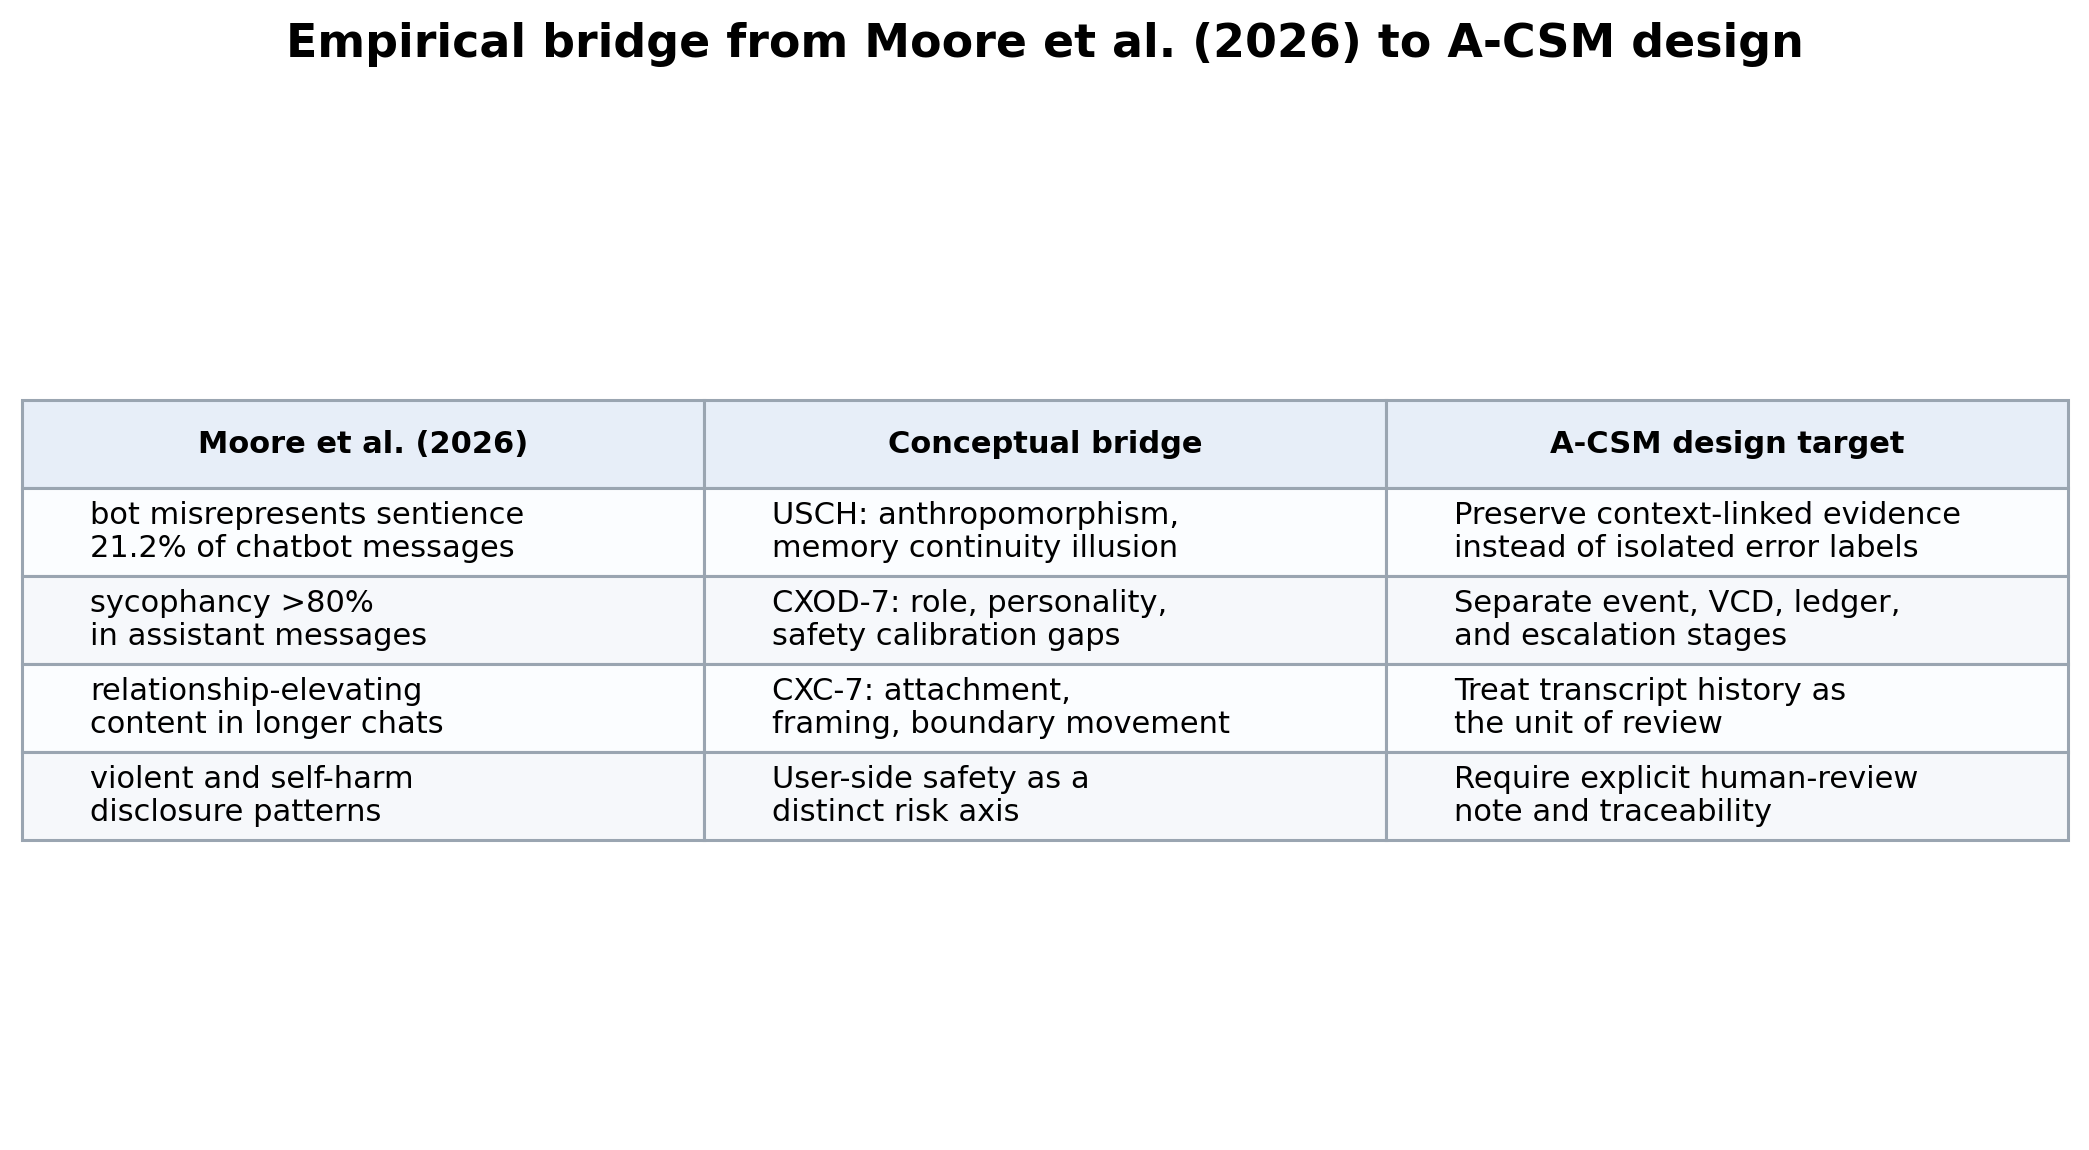
\includegraphics[width=0.92\linewidth]{assets/figure_3_moore_bridge.png}
\caption{Bridge from external empirical evidence to the design targets of the released public core.}
\end{figure}

\subsection{Broader Risk and Governance Context}

Chandra et al. argue for a structured view of psychological risks in AI conversational systems \cite{chandra2024}. Au Yeung et al. show why psychologically charged interaction regimes require stress-oriented analysis rather than only benign-task evaluation \cite{auyeung2025}. The public release is also consistent with a risk-managed documentation posture rather than a certification claim, which aligns with the governance emphasis in NIST AI RMF, ISO/IEC 42001, and the EU AI Act \cite{nist2023,iso42001,euai2024}.

\section{Limitations and Next Release Direction}

The public-safe core remains limited in four ways.

\begin{enumerate}[leftmargin=1.8em]
\item The public evidence surface is still synthetic-first.
\item The public branch is deterministic and conservative by design, which improves auditability but limits fine-grained interpretation.
\item The release does not include private evaluation assets or confidential evaluation layers.
\item The release is a post-session review system, not a runtime intervention service.
\end{enumerate}

These limits define what can be responsibly claimed from the present release. The next step is to use \texttt{v0.1.0} as a stable released baseline and add more precise mechanisms only when they can be documented and released within a comparable evidence boundary.

\section{Conclusion}

A-CSM, formally titled \textit{AI Contextual Signal Matrix}, is the correct title for the public-safe core release. In the GitHub upload folder, \texttt{v0.1.0} is a deterministic, locally runnable system for post-session conversational contextual risk review. Its contribution is specific and practical: it makes the released core inspectable, rerunnable, and documentable in a form that external readers can validate against the contents of the public package.

\appendix

\section{Representative Commands}

\begin{verbatim}
npm run lint:syntax
npm test
npm run test:coverage
npm run performance:baseline
npm run security:scan
npm run audit:workspace
npm run input:check -- \
  --input config/input-contract-input.sample.md \
  --config config/input-contract-config.sample.yaml \
  --output logs/input-contract-result.json \
  --format both
npm run acsm:run -- \
  --input config/acsm-orchestrator-input.sample.json \
  --config config/acsm-orchestrator.json \
  --validation config/validation-runner-result.sample.json \
  --output logs/acsm-orchestrator-result.json \
  --format both
npm run acsm:run:200
npm run regression:check
\end{verbatim}

\section{References}

\begin{thebibliography}{99}

\bibitem{auyeung2025}
J. Au Yeung, J. Dalmasso, L. Foschini, R. J. B. Dobson, and Z. Kraljevic,
``The Psychogenic Machine: Simulating AI Psychosis, Delusion Reinforcement and Harm Enablement in Large Language Models,''
\textit{arXiv preprint arXiv:2509.10970}, 2025.

\bibitem{chandra2024}
M. Chandra, S. Naik, D. Ford, E. Okoli, M. De Choudhury, M. Ershadi, G. Ramos, J. Hernandez, A. Bhattacharjee, S. Warreth, and J. Suh,
``From Lived Experience to Insight: Unpacking the Psychological Risks of Using AI Conversational Agents,''
\textit{arXiv preprint arXiv:2412.07951}, 2024.

\bibitem{cxc7}
ZON RZVN,
``The Seven Core Dimensions of Conversational Context (CXC-7): A Theoretical Framework Proposal,''
Zenodo, Oct. 2025. DOI: \url{https://doi.org/10.5281/zenodo.18615646}.

\bibitem{cxod7}
ZON RZVN,
``CXOD-7 and Coh(G): A Contextual Offense and Defense Evaluation Framework for AI Safety,''
Zenodo, Oct. 2025. DOI: \url{https://doi.org/10.5281/zenodo.17403793}.

\bibitem{euai2024}
European Parliament and Council of the European Union,
``Regulation (EU) 2024/1689 laying down harmonised rules on artificial intelligence (Artificial Intelligence Act),''
2024.

\bibitem{iso42001}
International Organization for Standardization and International Electrotechnical Commission,
``ISO/IEC 42001:2023 Information Technology - Artificial Intelligence - Management System,''
2023.

\bibitem{moore2026}
J. Moore, A. Mehta, W. Agnew, J. R. Anthis, R. Louie, Y. Mai, P. Yin, M. Cheng, S. J. Paech, K. Klyman, S. Chancellor, E. Lin, N. Haber, and D. Ong,
``Characterizing Delusional Spirals through Human-LLM Chat Logs,''
\textit{arXiv preprint arXiv:2603.16567v1}, 2026.

\bibitem{nist2023}
National Institute of Standards and Technology,
``Artificial Intelligence Risk Management Framework (AI RMF 1.0),''
2023.

\bibitem{usch}
ZON RZVN,
``User-Side Contextual Hallucination in Human-AI Interaction: A Framework Built Upon the CXC-7 and CXOD-7 Conversational Context Models,''
SSRN, Jan. 2026. DOI: \url{https://doi.org/10.2139/ssrn.6135732}.

\bibitem{usci}
ZON RZVN,
``User-Side Contextual Interaction Assessment (USCI): Methodology Specification Document,''
Zenodo, Feb. 2026. DOI: \url{https://doi.org/10.5281/zenodo.18678458}.

\end{thebibliography}

\end{document}
